\section{Block creation}
\label{design:block_creation}

\subsection{Exchanging signatures protocol}
Nodes will exchange signatures on a common payload that contains the reputation metrics.
A simple design would be to let the initiator node $A$ send a payload to $B$.
The payload contains a claim on an increase of reputation and a signature made by $A$.
If the node $B$ accepts the claim of the increase in reputation,
then he will add his own signature to the claim.
The payload and the two signatures are now a new block.
The block will be added to the current chain of node $B$ 
and the block will be sent to node $A$ to be appended to the chain of $A$.

This simple design does have one major problem.
It can never be decided in an asynchronous communication model
if the other node will ever respond and when it will respond.
The proposed block by $A$ only needs an interaction of $B$ to be finished
and $B$ can finish this transaction at anytime that he decides upon.

But the future block contains an immutable hash pointer
to the previous block in the chain of node $A$.
So while this transaction for a potential block is outstanding,
node $A$ cannot interact with any other node $C$ to create a different block.
If it would, then if $B$ could ultimately respond and a branch with different blocks
would be created for the chain of $A$.
This simple design introduces therefor an external response dependency problem.

The to-be-designed system has to be fault tolerant to 
common problems in a challenged network, such as node failure.
A second design goal is to be able to process transactions quickly and on a large scale.
These design goals prevent the adaption of a simple design that will halt until node $B$ responds.
There are several possible designs that are a solution to this problem.

\subsubsection{Fair exchange signature scheme}
A fair exchange signature scheme (FESS) allows two players to exchange digital signatures in a fair way.
Fair constitutes that no player can take advantage of the other.
Either both players receive each others signature or no player receives the other's signature.
It is infeasible for a node to acquire a signature without giving up their own signature.\cite{asokan-fairexchange}.
A FESS could be implement for the fair creation of the block.

But all known current FESSs use a trusted third party (TTP) at some point\cite{asokan-fairexchange}.
Some schemes exist that are optimistic and will only need a TTP to resolve conflicts.
But any TTP will not adhere to the Tribler philosphy 
of being a truly fully distributed peer-to-peer system.
The TTP will introduce a single point of trust and a scalability bottleneck.

\subsubsection{Reverse repairing of chain}
Another potential solution would be to rework part of the chain.
The creation of block could be deemed to have failed by node $A$.
If at a later point the block is still created by $B$,
then this situation can be handled by node $A$ in two possible ways.

The block could be reworked back into the chain.
This would require every hash pointer to be updated afterwards.
If these hash pointers are modified, then the signatures are invalid.
Every signature would have to be renewed and requested at every node.
This can become unscalable if nodes needs to rework many blocks and can clog the system.
These nodes can possible no longer respond and would result in new invalid blocks.

\subsubsection{Half signed blocks}
The chosen solution is to keep it simple and allow for inconsistencies between the chains of $A$ and $B$.
It will be shown that if an inconsistency does occur this is in favor of $A$.

When node $A$ sends a signature request to $B$,
then $A$ will be optimistic and will wait for $B$ for a timeout period.
During this time $A$ will not interact with another node $C$.
But if $A$ does not have to interact with node $C$ after the timeout period,
then $A$ will still accept a response of $B$.
There are three potential scenario's of what will happen to the message.

\begin{enumerate}
\item
In the normal situation node $B$ will respond in time to the message.
$B$ will send back the message
and both $A$ and $B$ will have added the same block in their own chains.
This situation also occurs if $A$ has timed out,
but has not yet interacted with another node $C$.

\item
Node $B$ can be malicious or simply have failed and $B$ will never respond.
Node $A$ will timeout and can continue interacting with other nodes $C$.
Next to this, node $A$ will have to decide how to react upon $B$ not responding.
A possibility would be to stop helping $B$.

\item
The response of $B$ can also be late.
After $B$ has received the request by $A$,
$B$ will create a block and adds this block to his chain.
$B$ will send his response to $A$,
but the message will arrive too late at $A$.
$A$ will ignore the message and not add the block to his chain,
\end{enumerate}

The last scenario is the most complex and requires additional clarification.
$A$ initiates the signature request and therefor the block will be favourable for his reputation.
Because this is a reputation system, this inconsistency is an allowable comprimise.
In a currency system, this comprimise would not be allowable.

$A$ can not later append the late block from $B$,
because the previous hash of $A$ will be used in a new block describing an interaction with $C$.
The late block demonstrates 

The design is scalable as it will not block too long waiting for a failed node 
and will try to interact as fast as possible with other nodes.
A small grace period can be used to allow node $B$ to have enough time to respond in a normal manner.
No trusted third party is introduced so a distributed design is achieved.

\subsection{Dispersy}
Dispersy is middleware for data dissemination in a network.
Dispersy is used heavily within Tribler
and is also the core library MultiChain has been build upon.
Dispersy can also be used to exchange data between two specific nodes \cite{zeilemaker-dispersy}.
Dispersy is used to exchange messages between nodes implementing MultiChain.

\subsection{Adding append functionality}
Within Dispersy functionality was already build to create a message, sign the message
and request multiple nodes to also provide their signature on this message.
This existing functionality could be used by MultiChain to exchange signatures
between Alice and Bob for the creating of a new block.

Alice would initiate a message, insert her data into this message, sign the message, and send this message to Bob.
The functionality would allow Bob to accept the message and provide his signature or
modify the message and provide his signature.

Only Bob knows the hash of his head node, and the total up and total download metrics.
So Bob will always modify the message and insert his own data in the message.
But this would invalidate the signature of Alice,
because the signature of Alice was also placed on the empty part of the message.
The contents of the message and who signs what can be seen in Figure \ref{fig:payload-signature-old}.

\begin{figure}
	\centerline{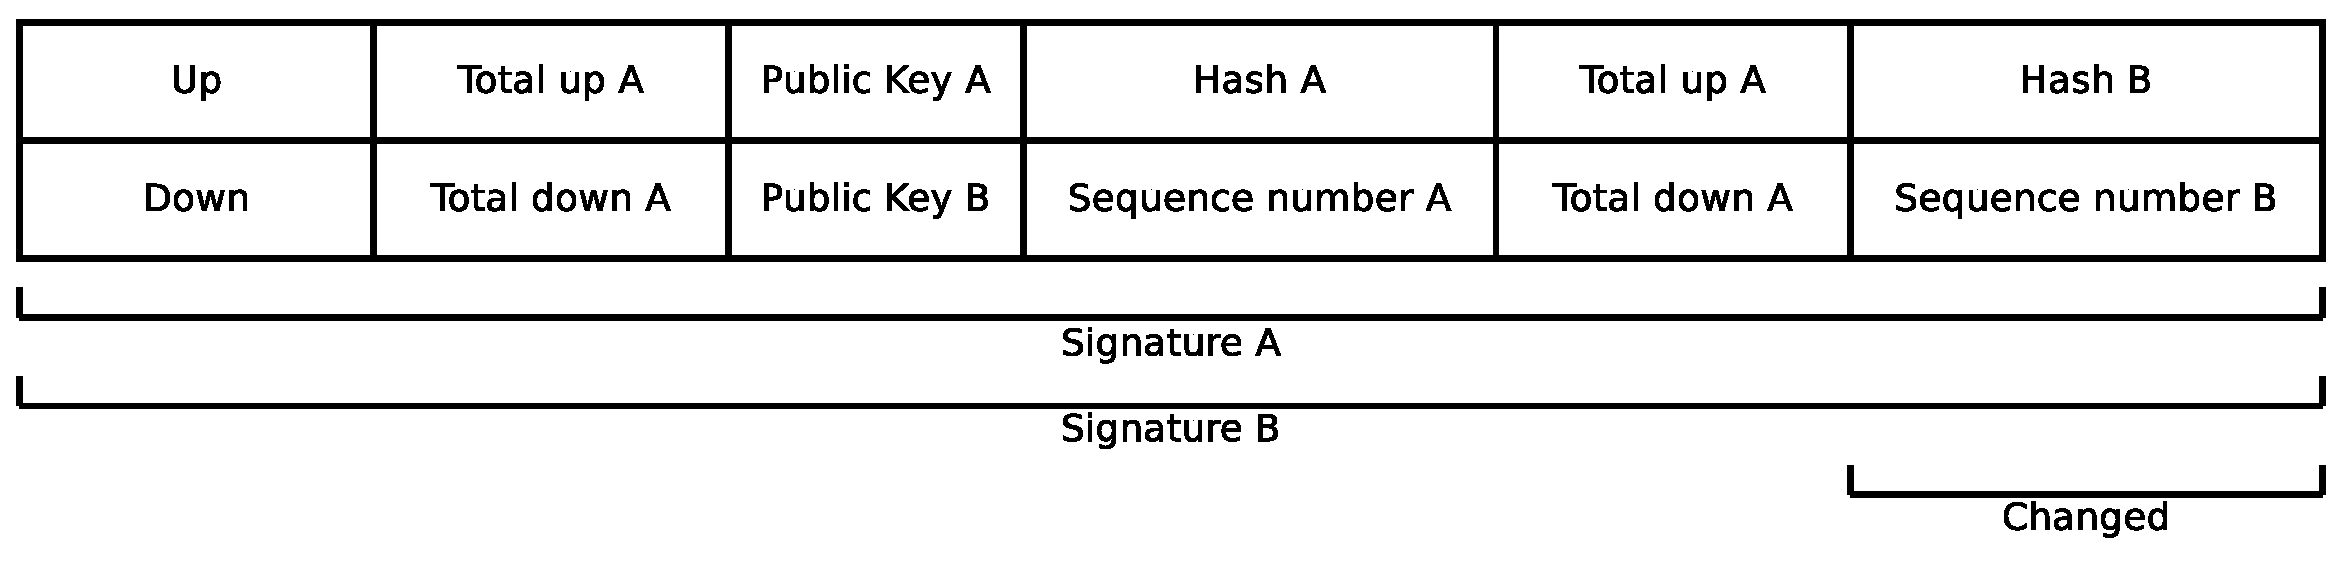
\includegraphics[scale=0.3]{design/figs/signature_old.eps}}
	\caption{Payload and signature using existing functionality.}
	\label{fig:payload-signature-old}
\end{figure}

After Bob returns the message,
Alice would have to resign the message.
But Bob also needs this valid signature from Alice before he can add the block to his own chain.
So Alice would need to send a third message to with the new, valid signature back to Bob.
A sequence diagram can be seen in Figure \ref{fig:exchange-old-sequence}.

\begin{figure}
	\centerline{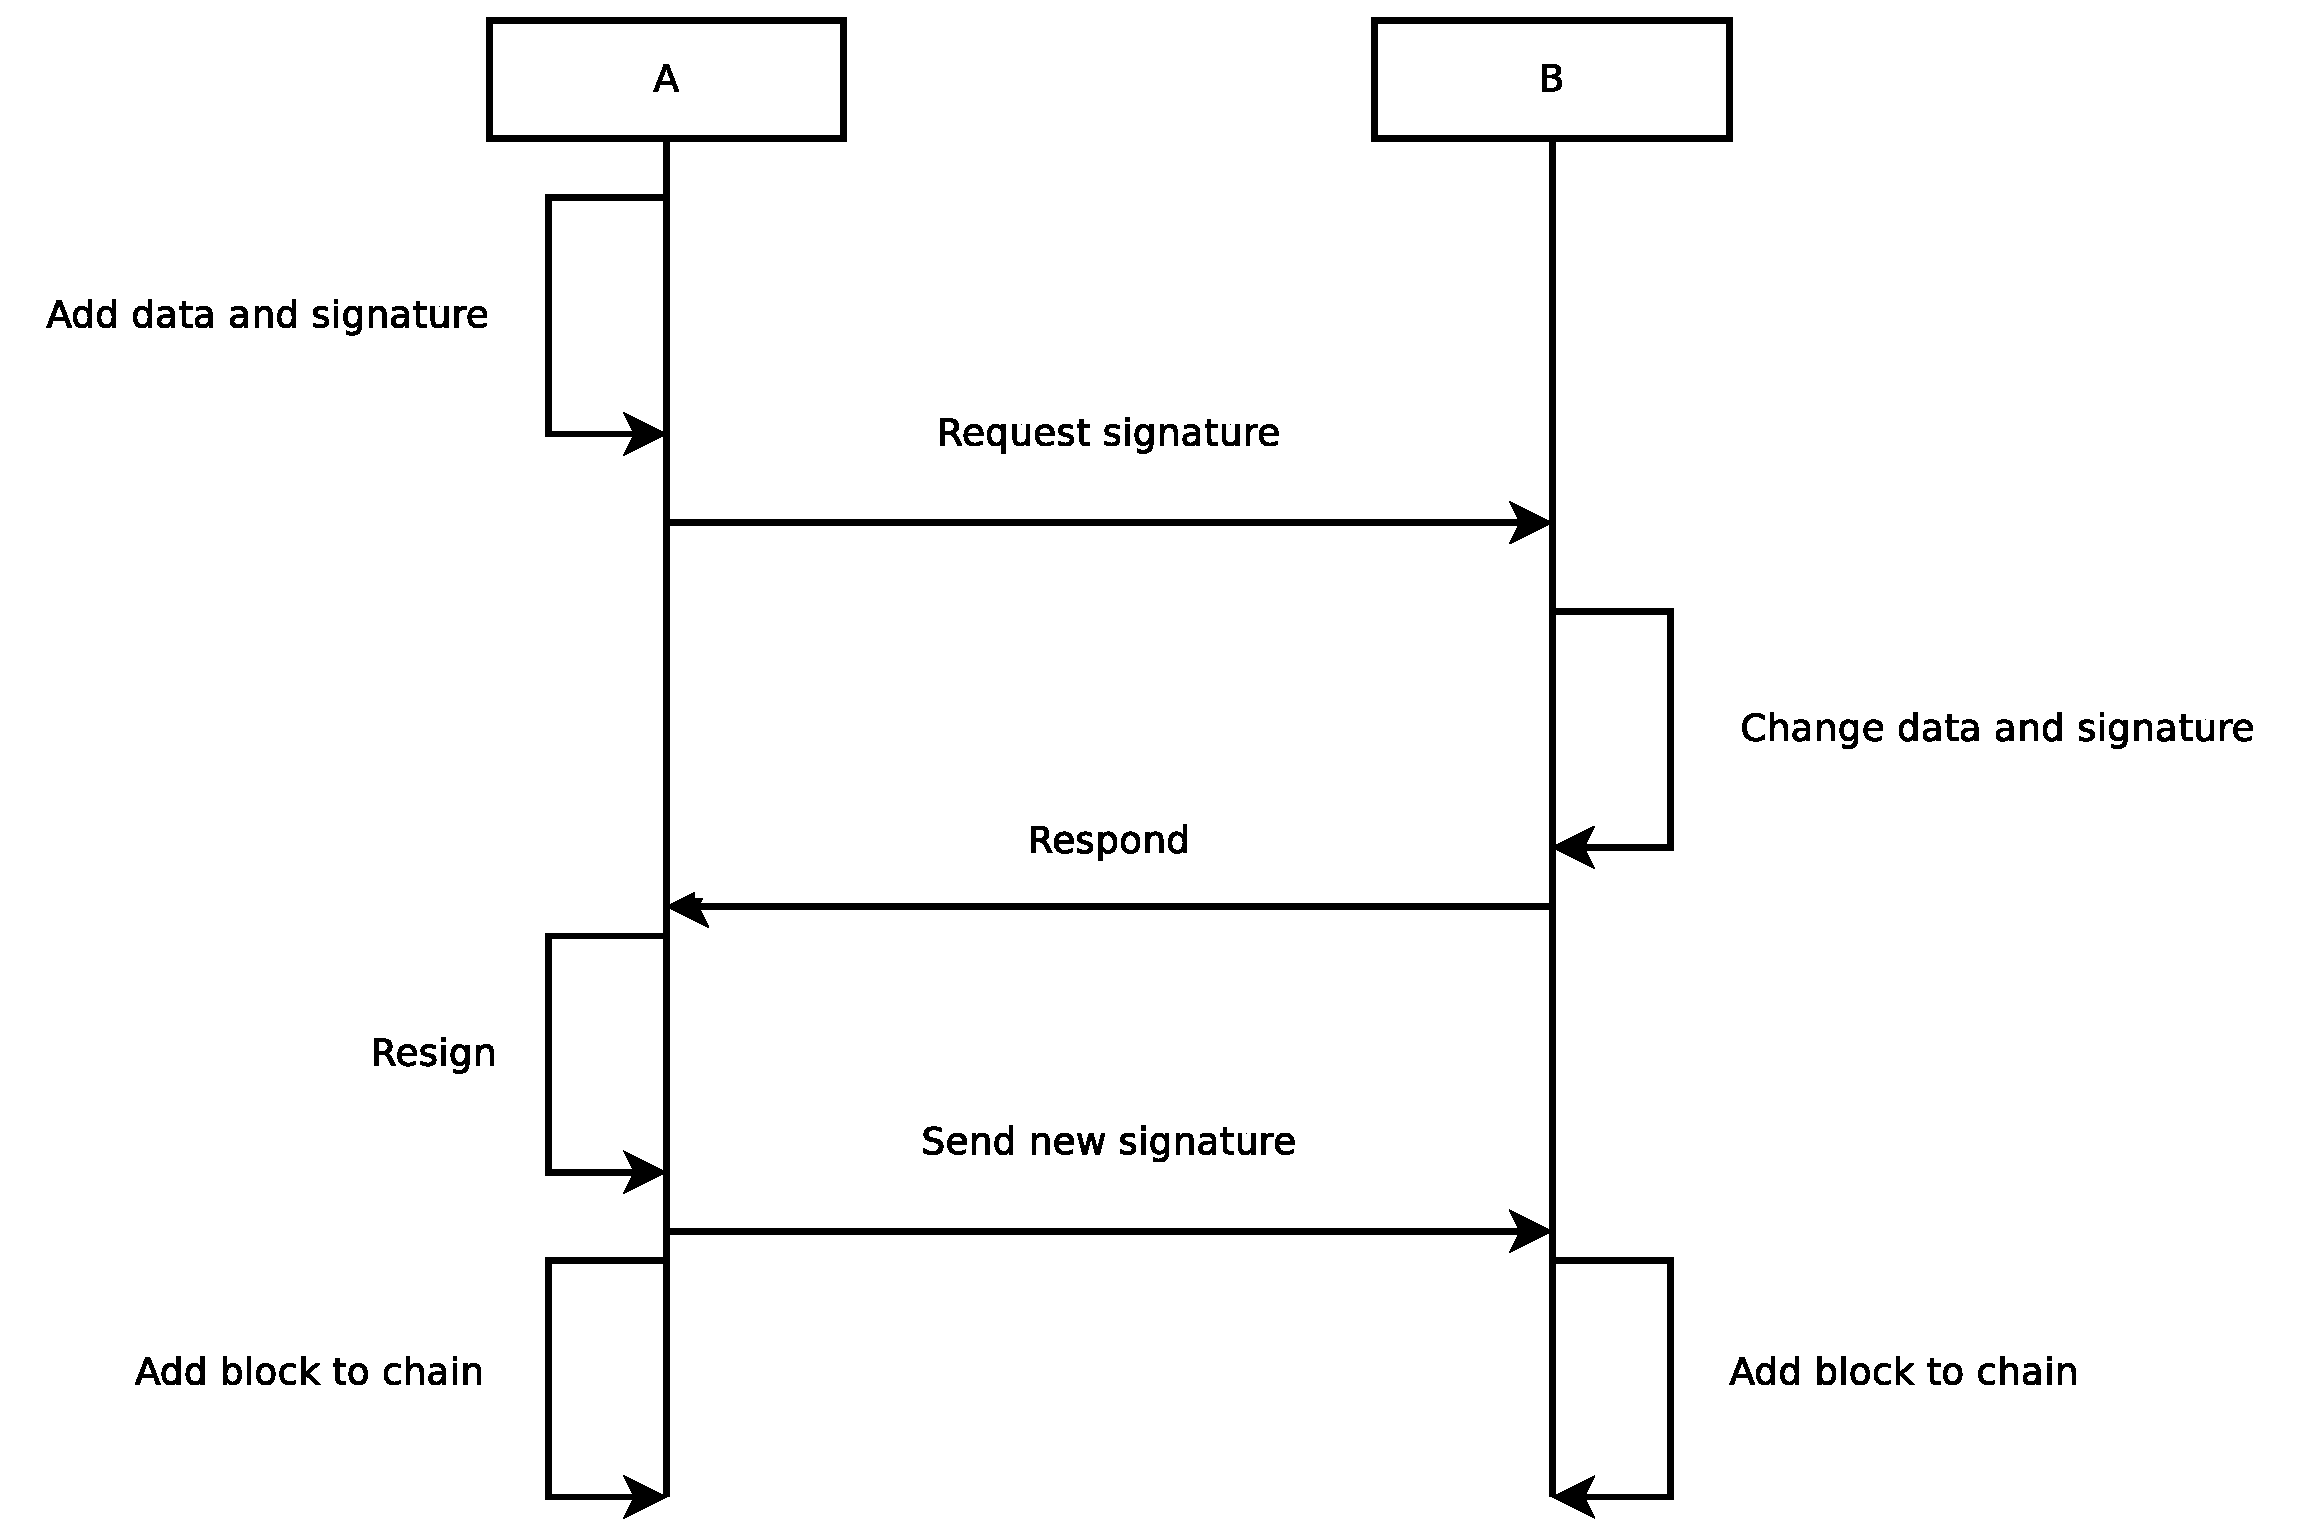
\includegraphics[scale=0.3]{design/figs/exchange_old.eps}}
	\caption{Exchanging signatures using existing functionality.}
	\label{fig:exchange-old-sequence}
\end{figure}

Alice can only make valid claims about and have authority over the interaction between her and Bob.
So she does not need to sign the data containing the previous hash and the total up and down of Bob.
This property allows Bob to append his own data to that of Alice.
Alice's signature would not become invalid.
Functionality was added to Dispersy that allows to append data in a signature request.
The parts of what is signed by Alice and Bob can be seen in Figure \ref{fig:payload-signature-new}.

\begin{figure}
	\centerline{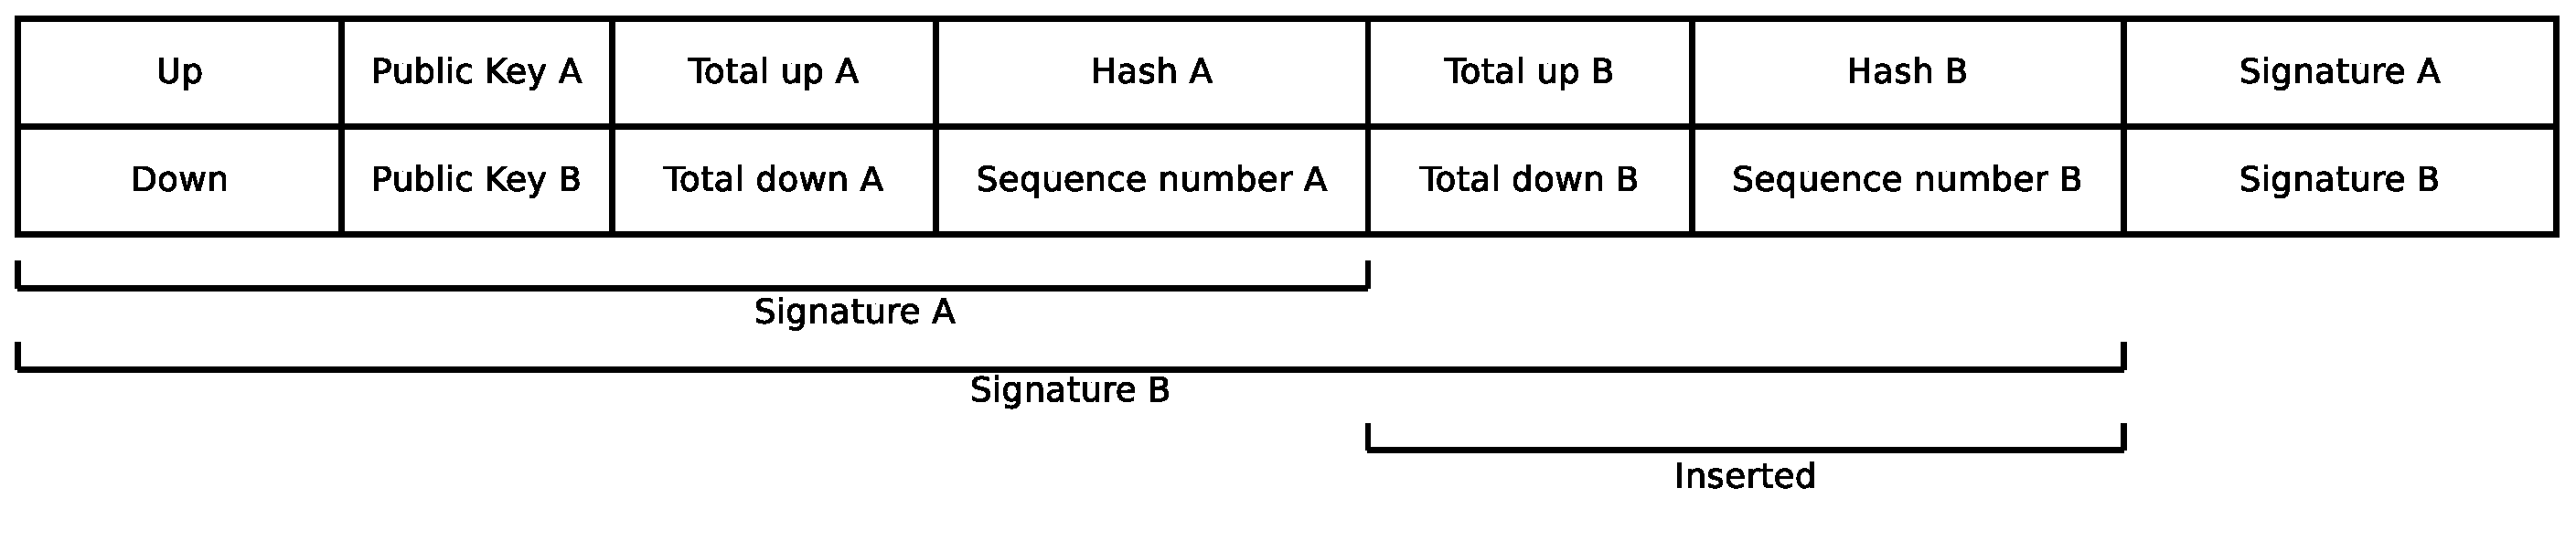
\includegraphics[scale=0.3]{design/figs/signature_new.eps}}
	\caption{Payload and signature using new functionality.}
	\label{fig:payload-signature-new}
\end{figure}

This allows the full signature exchange to be achieved within two messages.
Alice creates a message to Bob, but only signs her data.
Bob inserts his data upon arrival and signs everything.
Bob saves this message as a block to his own chain
and sends the message back to Alice.
Upon arrival Alice can also convert the message to a new block and add this to her own chain.
Now only two messages are between Alice and Bob are necessary.
The new sequence diagram can be seen in Figure \ref{fig:exchange-new-sequence}.

\begin{figure}[tbp]
	\centerline{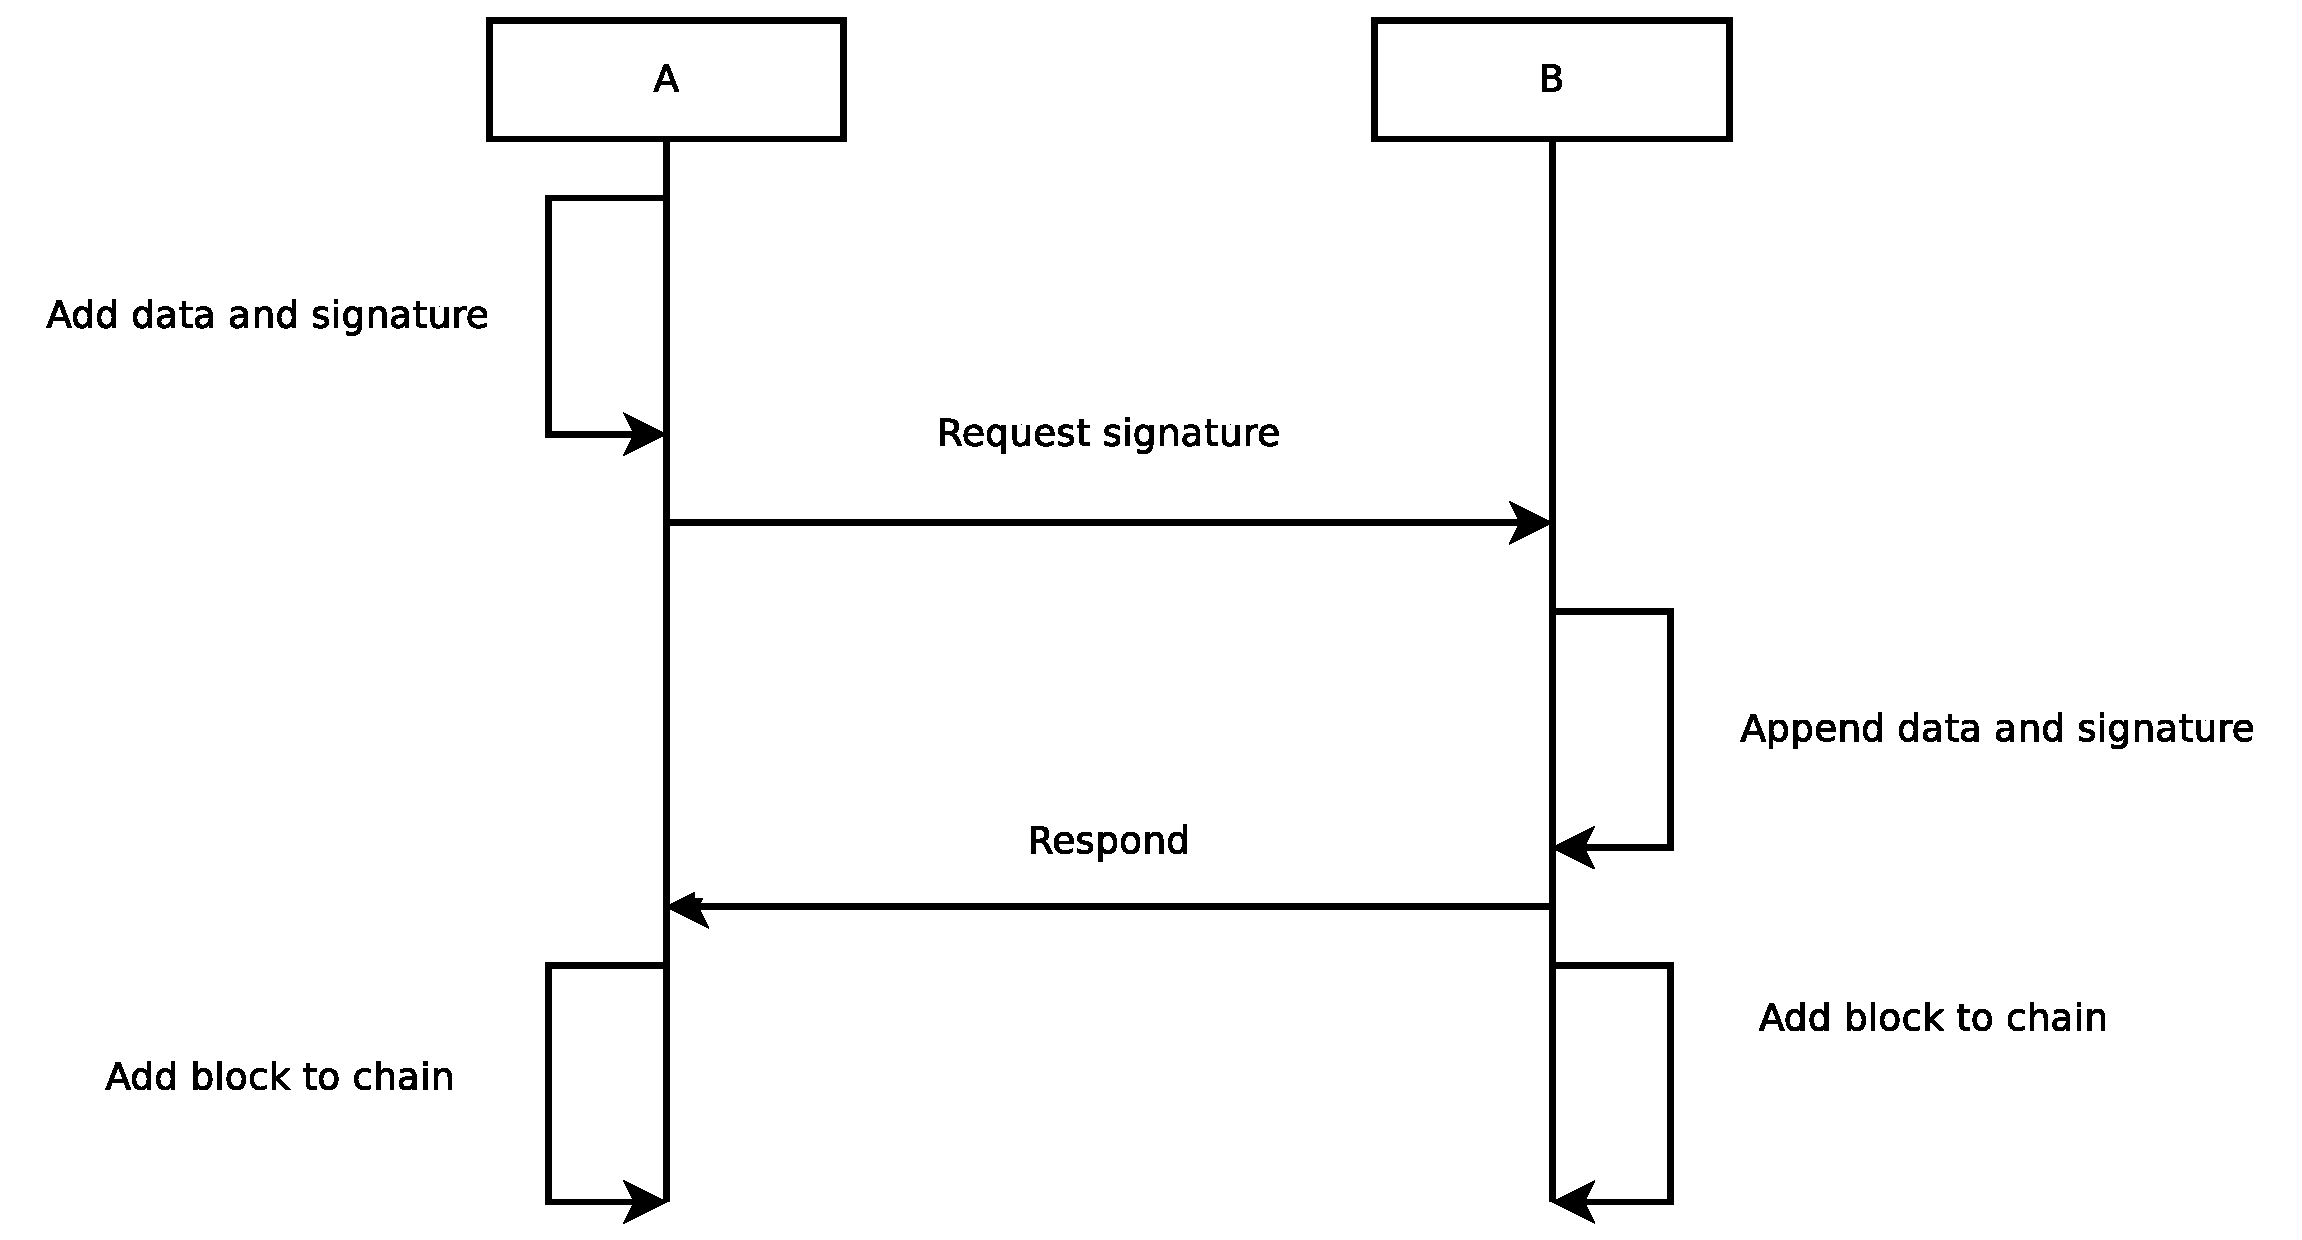
\includegraphics[scale=0.3]{design/figs/exchange_new.eps}}
	\caption{Exchanging signatures using added functionality.}
	\label{fig:exchange-new-sequence}
\end{figure}

\subsection{Block size}
The size of a block is important as it determines how fast the total size of a chain will grow
and the utilization of the bandwidth of network to transfer blocks.
The size is dependend on the size of the parts of the blocks
and can be determined by the choice of cryptographic primitives.
Hashing function turn a variable message string to a fixed size message digest\cite{VanderLubbe-crypto}.
The fixed size is dependend on the choice of hashing function.
Similair cryptographic signing functions deterimine the size of a signature.
An overview of the size of the parts of a block can be seen in Table: \ref{table:block_size}.
The total size of a block is 240 bytes.

\begin{table}[]
\begin{adjustwidth}{-.5in}{-.5in}
\begin{center}
\begin{tabular}{l|lll|ll}
Name              & Type             & Bytes                   & Name              & Type             & Bytes \\ \hline
Uploaded KBytes   & integer          & \multicolumn{1}{l|}{4}  & Downloaded Bytes  & integer          & 4     \\
Total Up A        & integer          & \multicolumn{1}{l|}{4}  & Total Up B        & integer          & 4     \\
Total Down A      & integer          & \multicolumn{1}{l|}{4}  & Total Down B      & integer          & 4     \\
Prior Record A    & SHA1 digest      & \multicolumn{1}{l|}{20} & Prior Record B    & SHA1 digest      & 20    \\
Sequence Number A & signed integer   & \multicolumn{1}{l|}{4}  & Sequence Number B & signed integer   & 4     \\
Public Key A      & EC binary format & \multicolumn{1}{l|}{64} & Public Key B      & EC binary format & 64    \\
Signature A       & EC signature     & \multicolumn{1}{l|}{40} & Signature B       & EC signature     & 40
\end{tabular}
\caption{Block size}
\label{table:block_size}
\end{center}
\end{adjustwidth}
\end{table}

MultiChain differs from Bitcoin in that a single block contains only one transaction.
In Bitcoin a block can contain several transactions up to a certain maximum.
The blocks are created directly between nodes containing a transaction
that will transcribe the interaction between A and B.